\documentclass[a4paper,12pt]{article}
% \usepackage[utf8]{inputenc}
\usepackage{parskip}
% \usepackage[sorting=none]{biblatex}
% \usepackage{url}
\usepackage{epsfig}
\usepackage{graphics}
\usepackage{fancyhdr}

\usepackage{mathtools}
% \usepackage{graphicx}
\usepackage[justification=centering]{caption}
\usepackage{caption}
\usepackage{subcaption}
\usepackage{amssymb}
\usepackage{amsmath}
\usepackage{tabularx}
\usepackage{xcolor}
\usepackage{multirow}
\usepackage{graphicx}
\usepackage{xcolor}
\usepackage{arydshln}
\usepackage{tikz}
\usetikzlibrary{shapes.geometric, arrows}


\newcommand*{\progName}[1]{\mbox{\texttt{#1}}}

\usepackage{geometry}
\geometry{
  paper=a4paper,
  margin=54pt,
  includeheadfoot
}

% \documentclass{amsart}

% \usepackage[margin=1in]{geometry}        
\usepackage[utf8]{inputenc} % allow utf-8 input
\usepackage[T1]{fontenc}    % use 8-bit T1 fonts
\usepackage{hyperref}       % hyperlinks
\usepackage{url}            % simple URL typesetting
\usepackage{booktabs}       % professional-quality tables
% \usepackage{amsfonts}       % blackboard math symbols
\usepackage{nicefrac}       % compact symbols for 1/2, etc.
\usepackage{microtype}      % microtypography
\usepackage{amsmath,amsfonts,amssymb}
% \usepackage{todonotes}

\usepackage{algorithm}
\usepackage{algpseudocode}

\usepackage[english]{babel}
\newtheorem{theorem}{Theorem}
\usepackage{soul}

\DeclareMathOperator*{\argmax}{arg\,max}
\DeclareMathOperator*{\argmin}{arg\,min}

%package for references
\usepackage[backend=biber, style=alphabetic, sorting=anyt]{biblatex}
\usepackage{csquotes}

\addbibresource{sources.bib}


\title{Pacman capture the flag \\ Assignment 4 Report}

\author{\hspace*{-0.5cm}
GROUP 03\\
\begin{tabular}{cccc}
Shekhar Devm Upadhyay & Aiman Shenawa\\
20010531 & 001021 \\
sdup@kth.se & ashenawa@kth.se \\
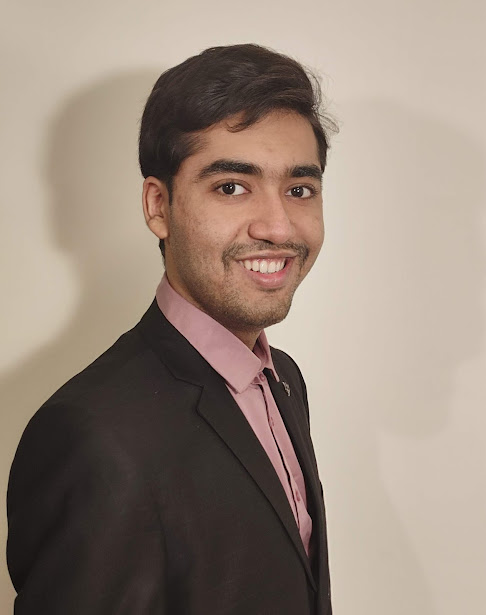
\includegraphics[width=0.2\linewidth]{side_profile.jpg} & 
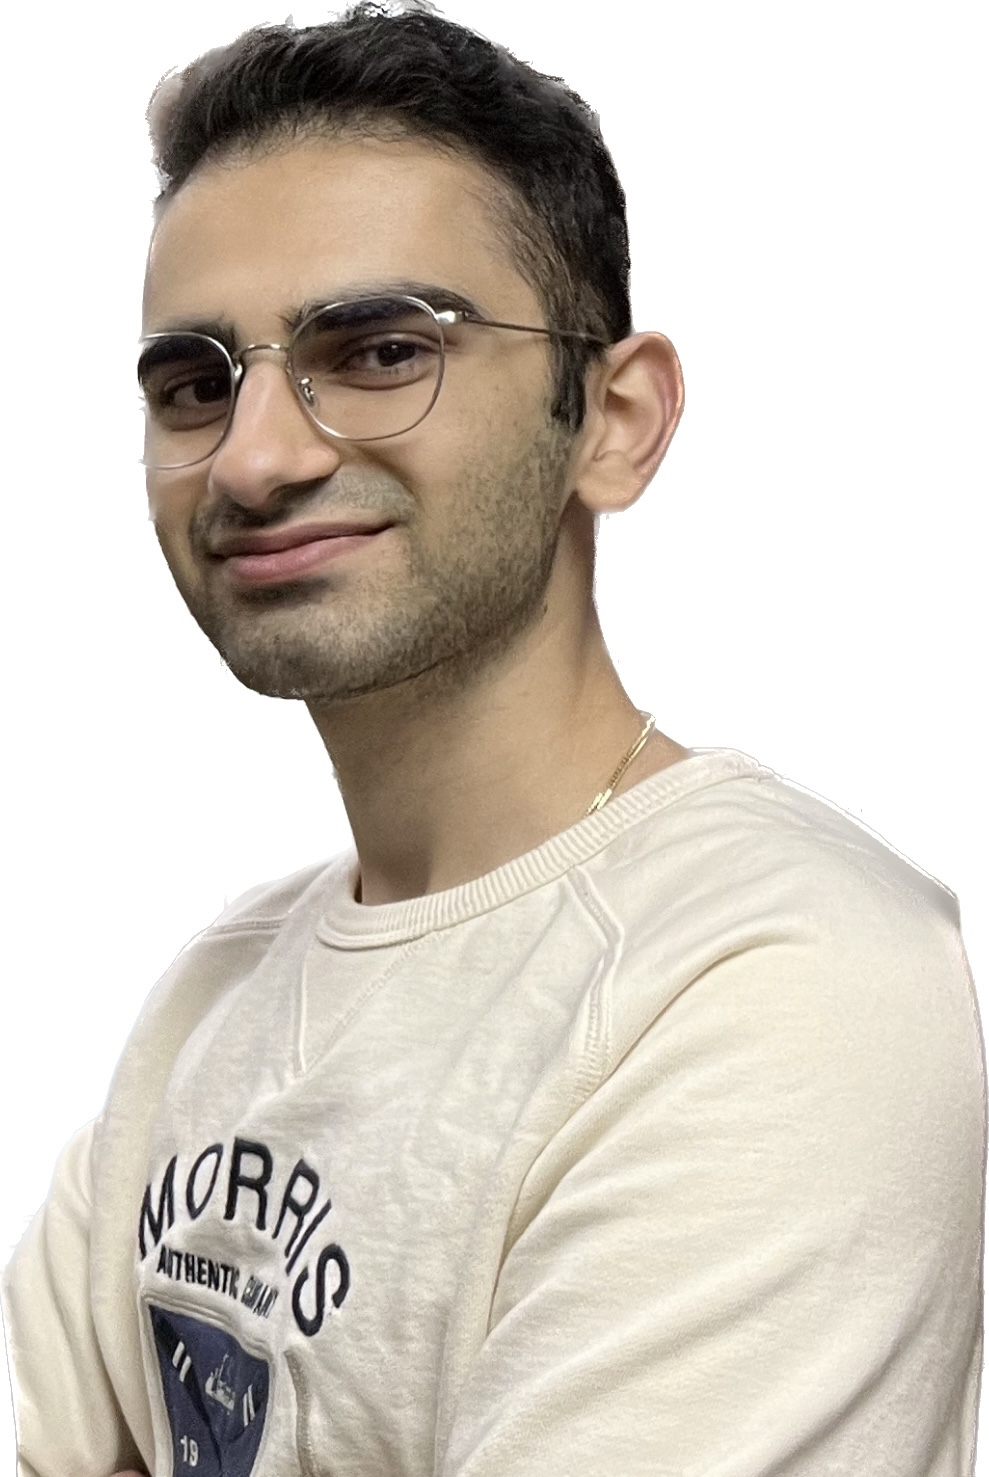
\includegraphics[width=0.17\linewidth]{Aiman_picture.jpg}
\end{tabular}} 
\date{May 2023}

% \pagestyle{fancy}
\setlength{\headheight}{15pt}
\fancyhf{}
\lhead{DD2438} % DO NOT REMOVE!!!!
\rhead{Shekhar Devm Upadhyay, Aiman Shenawa} %% UPDATE WITH YOUR NAMES

\addbibresource{sources.bib}

\begin{document}

\maketitle
\thispagestyle{fancy}

\begin{abstract}
% Describe the problem and importance in detail
% why it is important to study

% introduce pacman capture the flag problem







\end{abstract}
\clearpage

%% REMEMBER TO WRITE IN A TOP-DOWN FASHION, STARTING EACH SECTION WITH A SUMMARY. 

\section{Introduction}
% Describe the problem and importance in detail

Pacman capture the flag is a project developed by UC Berkely, it is a challenge that combines classic video game mechanics with artificial intelligence techniques. 
The goal of the project is to develop an agent that can play the game of Pacman capture the flag. The game is played on a grid, where the agent can move in four directions, up, down, left and right. 
The grid is split into two halves, in each half there is a team of Pacman agents, the goal of the game is to capture the food pellets from the other team's side and bring them back to your side while also preventing the other team from doing the same.














\subsection{Task Description}

This report will discuss ....




These problems and their solutions are addressed in further detail in the following section \ref{rel_work}.




\subsection{Contribution}
% Describe the contribution of the report in detail









\subsection{Outline}











\section{Related Work}
\label{rel_work}
% Describe the related work in detail

This section will discuss the related work in detail. 




\subsection{Collision Avoidance}
\label{rel_work_collision}

\paragraph{Relevance of the Problem}


















\section{Method}
\label{method}
% Proposed method section explaining what you did in more detail

In this section, we will discuss ...





\section{Experiments and Results}
\label{sec:experiments_and_results}

% mention failure to clear intersection with cars
First, we will describe the experimental setup for the two problems, and then we will present the results for each of the problems separately.

\subsection{Experimental Setup}
\label{subsec:experimental_setup}
% Containing the results of other groups in a table, 
The experimental environment was largely dependent on the problems. Both problems shared a a similar map and obstacle structure, the main difference being the agent objectives, environment sizes, and the fact that we didn't have any obstacles in the soccer environment (except, of course, for the boundaries of the field). For each of the problems, we were to compute and pass a set of inputs to the agents (different based on whether the agent was a car or a drone). The agents moved based on the provided input, and the updated positions and velocities were used in the next timestep to compute the next set of inputs. The agents were also provided with a set of parameters that decided how the different forces were weighted. The parameters were tuned by hand separately for each type of agent, and were not changed during the course of the simulation.

All the solutions for Collision Avoidance were repeatedly tested in the Unity game environment on three terrains: an open field, an intersection, and a random map. The open field was a simple map with no obstacles. The intersection was a map with a crossroad and a few obstacles. The random map was a map with randomly generated obstacles. There were two possible initializations for the positions of the agents: first, in a circular formation, and second, in a random formation. The solutions were tested in the Unity game environment with $50$ agents. Based on performance, the solutions were improved and adjusted in an iterative manner.


\subsection{Results}
\label{subsec:results}
In this section, we summarize the results of our experiments. We first present the results of the Collision Avoidance problem, and then present the results of the Soccer problem. We then go on to discuss the merits and shortcomings of the best solutions from all the groups.









\section{Summary and Conclusions}




% \section{Future Work}









% \clearpage
% \newpage
\printbibliography

\newpage

\appendix
% print the appendix title on the top of the page
\section{Appendix}
\label{sec:appendix}








% \paragraph{Relevance of the Problem}
% Collision avoidance is a critical problem in multi-agent systems, where agents must work together to accomplish tasks in a shared environment, where the actions of one agent may affect the state of the environment and the other agents. In this context, collision avoidance is essential to ensure the safety of agents and the success of the mission. This has applications in various domains, including unmanned aerial vehicles, autonomous vehicles, and mobile robots. In these applications, agents must navigate through dynamic and crowded environments while avoiding obstacles and other agents. Thus, developing effective collision avoidance strategies is critical to the reliable and safe operation of multi-agent systems in real-world applications.




% In \cite{6606326}, a novel behaviour tree based control used in decision making processes of robot soccer is proposed.
% The most impressive point is passing.
% The passing behavior tree first controls two robots using parallel sequences, with the passer and receiver aligned, 
% and then the tree checks if the pass is safe. If the ball can be passed, the passer shoots the ball.
% Next, the sequence waits for the ball to start moving, and once this happens, 
% we again wait for the ball to stop, or for the ball to come within the diameter of the receiver's robot, 
% at which point the receiver moves and captures the ball. The use of BT approach allows to model complicated 
% situations easily that show advantages of this technique over finite state machines widely
% used in robot control\cite{6606326}.


% \begin{eqnarray}
%   \label{eqn:car_input}
%   \begin{aligned}
%     % atan(dot product of a and r)
%     \text{steering} &= \arctan(\overrightarrow{\mathbf{a}} \bullet \hat{\mathbf{r}}) \\
%     % atan(dot product of a and f)
%     \text{gas} &= \arctan(\overrightarrow{\mathbf{a}} \bullet \hat{\mathbf{f}}) \\
%     % if magnitude of gas is too small, scale it to 0.2. add a comment about epsilon at the end of the line
%     \text{gas} &= \text{gas} \cdot \frac{\epsilon}{\text{min}(|\text{gas}|, \epsilon)} \\
%     % \text{brake} &= 0 \\
%   \end{aligned}
% \end{eqnarray}

% % figure showing drag
% \begin{figure}[!htbp]
%   \centering
%   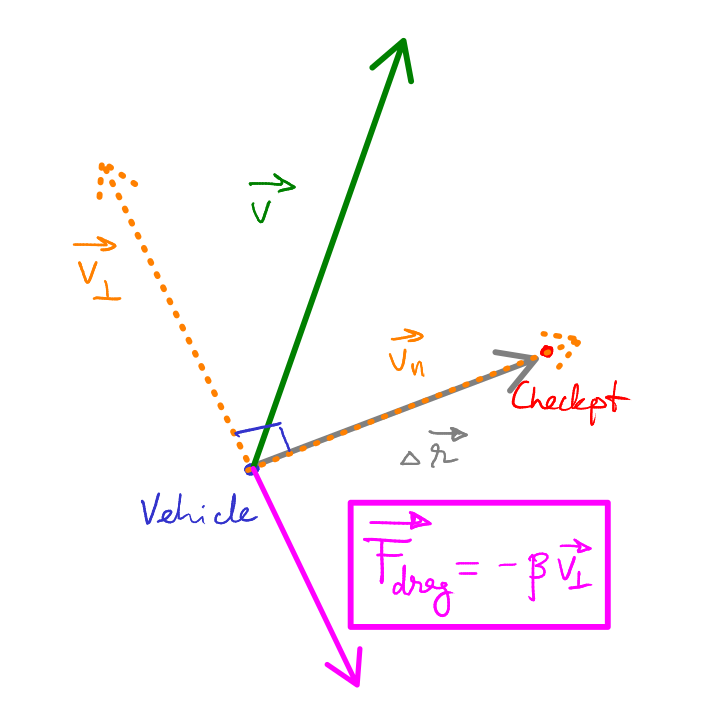
\includegraphics[width=0.3\textwidth]{./figures/intelli_drag.png}
%   \caption{Assistive drag force to help the agent maintain its reference trajectory.}
%   \label{fig:drag_force}
% \end{figure}

% % figure showing velocity obstacle
% \begin{figure}[!hptb]
%   \centering
%   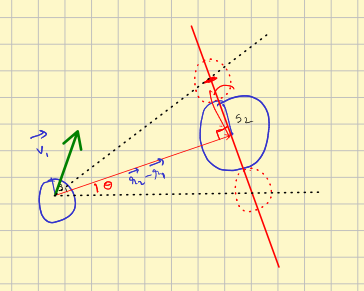
\includegraphics[width=0.3\textwidth]{./figures/VO_repulsion_setup.png}
%   \caption{Velocity Obstacle setup for two agents.}
%   \label{fig:velocity_obstacle_setup}
% \end{figure}


% table layout
% \begin{table}[!hptb]
%   \centering
%   \begin{tabular}{|c|c|c|c|c|c|c|}
%     \hline
%     \textbf{Terrain} & \multicolumn{2}{|c|}{\textbf{Open Field}} & \multicolumn{2}{|c|}{\textbf{Intersection}} & \multicolumn{2}{|c|}{\textbf{Unstructured}} \\
%     \hline
%     \textbf{Group} & \textbf{Circle} & \textbf{Random} & \textbf{Circle} & \textbf{Random} & \textbf{Circle} & \textbf{Random} \\
%     \hline
%     9 & 29 & 28.52 & 44 & 46 & 47 & 40.78 \\
%     \hline
%     13 & 34 & 47 & 55 & 47 & 50 & 47 \\
%     \hline
%     3 & \color{blue}{20.5} & \color{blue}{21} & \color{red}{287} & \color{blue}{32} & \color{blue}{30.5} & \color{blue}{26.5} \\
%     \hline
%     12 & 27.06 & 27.54 & 88.66 & 166.03 & 47.7 & 69.23 \\
%     \hline
%     10 & 42.8 & 42.9 & 64.6 & 158.42 & 52.05 & 69.88 \\
%     \hline
%     16 & 59.4 & 38 & 141.6 & 191.5 & 77.2 & 70.5 \\
%     \hline
%     \textbf{14} & 31.3 & 29.68 & 79.9 & 260.15 & 52.4 & 60 \\
%     \hline
%     \textbf{Overall Best Time} & 20.5 & 21 & 44 & 32 & 30.5 & 26.5 \\
%     \hline
%   \end{tabular}
%   \caption{Completion Times of the top 7 groups with drones on different terrains.}
%   \label{tab:results_drone_CA}
% \end{table}


% % figure showing pseudo traffic lights
% \begin{figure}[!hptb]
%   \centering
%   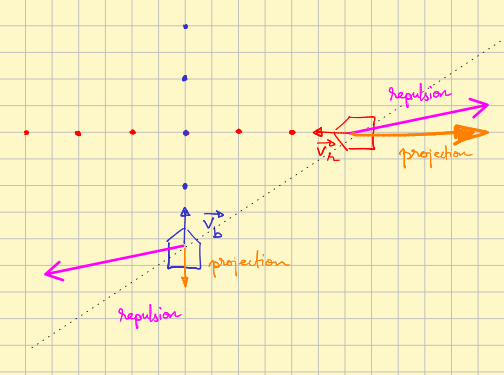
\includegraphics[width= 0.6\textwidth]{./figures/pseudo_traffic_lights.png}
%   \caption{Pseudo-traffic lights. Note that the repulsion force is only along the direction of the path. So the red car slows down a lot, while the blue car does not decelerate as much. The blue car can pass the intersection before the red car, without steering away from its original path.}
%   \label{fig:pseudo_traffic_lights}
% \end{figure}


% % figure showing ball chasing
% \begin{figure}[!hptb]
%   \centering
%   \begin{subfigure}[b]{0.45\textwidth}
%     \centering
%     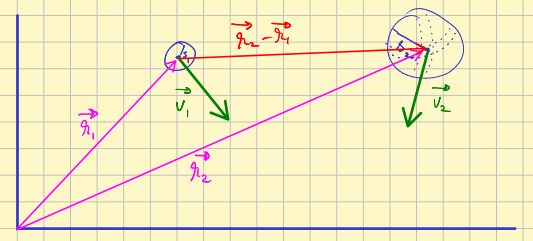
\includegraphics[width=\textwidth]{./figures/soccer_VO_attraction_setup.png}
%     \caption{VO\_Attraction Setting}
%     \label{fig:soccer_VO_attraction_setting}
%   \end{subfigure}
%   ~
%   \begin{subfigure}[b]{0.45\textwidth}
%     \centering
%     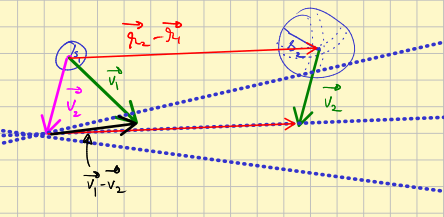
\includegraphics[width=\textwidth]{./figures/soccer_VO_attraction_setup_2.png}
%     \caption{VO\_Attraction Initial Setup}
%     \label{fig:soccer_VO_attraction_initial_setup}
%   \end{subfigure}
%   \caption{Setup for our Ball-chasing strategy.}
% \end{figure}



% table comparing results of different groups (drones)

% \begin{table}[!hptb]
%   \centering
%   \begin{tabular}{|c|c|c|c|c|c|c|}
%     \hline
%     \textbf{Terrain} & \multicolumn{2}{|c|}{\textbf{Open Field}} & \multicolumn{2}{|c|}{\textbf{Intersection}} & \multicolumn{2}{|c|}{\textbf{Unstructured}} \\
%     \hline
%     \textbf{Group} & \textbf{Circle} & \textbf{Random} & \textbf{Circle} & \textbf{Random} & \textbf{Circle} & \textbf{Random} \\
%     \hline
%     9 & 29 & 28.52 & 44 & 46 & 47 & 40.78 \\
%     \hline
%     13 & 34 & 47 & 55 & 47 & 50 & 47 \\
%     \hline
%     3 & \color{blue}{20.5} & \color{blue}{21} & \color{red}{287} & \color{blue}{32} & \color{blue}{30.5} & \color{blue}{26.5} \\
%     \hline
%     12 & 27.06 & 27.54 & 88.66 & 166.03 & 47.7 & 69.23 \\
%     \hline
%     10 & 42.8 & 42.9 & 64.6 & 158.42 & 52.05 & 69.88 \\
%     \hline
%     16 & 59.4 & 38 & 141.6 & 191.5 & 77.2 & 70.5 \\
%     \hline
%     \textbf{14} & 31.3 & 29.68 & 79.9 & 260.15 & 52.4 & 60 \\
%     \hline
%     \textbf{Overall Best Time} & 20.5 & 21 & 44 & 32 & 30.5 & 26.5 \\
%     \hline
%   \end{tabular}
%   \caption{Completion Times of the top 7 groups with drones on different terrains.}
%   \label{tab:results_drone_CA}
% \end{table}




\end{document}
